\section{Cel i założenia projektowe}
    \tab Powyższy projekt oparty jest o mikrokontroler z rodziny AVR: ATmega8A.
    Komunikując się z odpowiedniki sensorami jest w stanie zlokalizować się w przestrzeni,
    oraz stworzyć prostą mapę pomieszczenia, w którym się znajduje. A następnie swobodnie poruszać się po nim.

    \subsection{Środowisko sprzętowe}
        \tab Jak wyżej wspomniano, sercem projektu jest mikrokontroler ATmega8A, a wspomnianymi modułami są odpowiednio:
        \begin{enumerate}
            \item Ultradźwiękowa czujka odległości -- HC-SR04,
            \item Trój-osiowy akcelerometr -- ADXL345,
            \item Moduł bluetooth -- HC05,
            \item Scalony mostek H -- układ L293D TexasInstruments,
            \item Silniki modelarskie z przekładniami 1:48 o napięciu znamionowym 6V,
            \item Serwo mechanizm -- SG90.
        \end{enumerate}
% 
        Zasilanie dostarczają dwa wbudowane akumulatory litowo-jonowe 18650 o napięciu znamionowym 3.7V, podniesionym za pomocą przetwornicy STEP UP (CN6009) do około 5V.
        % Zasilanie jest z dwóch akumulatorów litowo-jonowych 18650 o napięciu znamionowym 3.7V, podniesionym za pomocą przetwornicy STEP UP do około 5V.


        \subsubsection{Schemat ideowy}
            Wstawić schemat
        
    \subsection{Środowisko programowe}
        \tab Program na ATmegę został napisany w języku C/C++, z wykorzystaniem bibliotek udostępnionych przez producenta.
        Do programowania, układu zostało wykorzystane narzędzie \textit{AVRdude} wraz z programatorem \textit{USBasp}.
        Natomiast graficzny interfejs dla komputerów klasy PC, został stworzony w Pythonie, z wykorzystaniem biblioteki ,,Turtle".

    \subsection{Interfejs komunikacyjny}
        \tab Wiele nowoczesnych urządzeń wykorzystuje rozmaite standardy i interfejsy komunikacyjne do różnych celów.
        Tak samo powyższy projekt wykorzystuje kilka prostych standardów do komunikacji zarówno z użytkownikiem oraz peryferiami.

        \subsubsection{Standard UART i interfejs bluetooth}
            \tab Podstawowym sposobem komunikacji z użytkownikiem jest protokół UART, wraz z interfejsem Bluetooth.
            Standard komunikacji UART, jest to prosty dwukierunkowy asynchroniczny sposób do przesyłania danych między dwoma urządzeniami.\\
            Opis ramki w standardzie UART:
            
            \begin{figure}[!h]
                \centering
                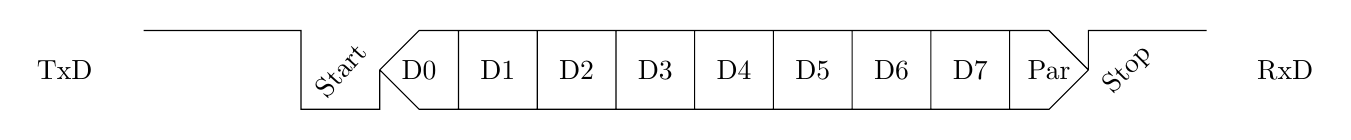
\begin{tikzpicture}
                    \draw
                    (-1, 0.5) node[]{TxD}
                    (0, 1) -- (2, 1)
                        -- (2, 0)
                        -- (3, 0)
                        -- (3, 0.5) coordinate(start) ++(-0.5, 0) node[rotate = 48]{Start}

                    (start) --++ (0.5, -0.5) -- ++ (8, 0) --++(0.5, 0.5) coordinate(stop)
                    (start) --++ (0.5, 0.5) -- ++ (8, 0) --++(0.5, -0.5)

                    (start) ++ (1, 0.5) -- ++ (0, -1) ++ (-0.5, 0.5) node[]{D0}
                    (start) ++ (2, 0.5) -- ++ (0, -1) ++ (-0.5, 0.5) node[]{D1}
                    (start) ++ (3, 0.5) -- ++ (0, -1) ++ (-0.5, 0.5) node[]{D2}
                    (start) ++ (4, 0.5) -- ++ (0, -1) ++ (-0.5, 0.5) node[]{D3}
                    (start) ++ (5, 0.5) -- ++ (0, -1) ++ (-0.5, 0.5) node[]{D4}
                    (start) ++ (6, 0.5) -- ++ (0, -1) ++ (-0.5, 0.5) node[]{D5}
                    (start) ++ (7, 0.5) -- ++ (0, -1) ++ (-0.5, 0.5) node[]{D6}
                    (start) ++ (8, 0.5) -- ++ (0, -1) ++ (-0.5, 0.5) node[]{D7}
                    (start) ++ (8.5, 0) node[]{Par}

                    (stop) --++(0, 0.5) -- ++(1.5, 0) coordinate(end)
                    (stop) ++ (0.5, 0) node[rotate = 45]{Stop}
                    (end) ++ (1, -0.5) node[]{RxD}
                        
                    ;
                \end{tikzpicture}
                \caption{Ramka danych w standardzie UART}
            \end{figure}

            Komunikacja, między urządzeniami odbywa się z szybkością 9600 baud'ów